\chapter{Πειραματική Αξιολόγηση}
\label{ch:Experimental Evaluation}
Οι διάφορες υλοποιήσεις που πραγματοποιήθηκαν στα πλαίσια της τρέχουσας διπλωματικής εργασίας αξιολογήθηκαν πειραματικά με τη χρήση μετροπρογραμμάτων (benchmarks) τόσο για την επιβεβαίωση της ορθότητας της υλοποίησης, όσο και για τη μέτρηση των επιδόσεων που επιτεύχθηκαν.


\section{Περιγραφή Συστημάτων}
\label{sec:Systems Description}
Η εκτέλεση των πειραμάτων έγινε σε δύο υπολογιστικά συστήματα τα οποία αντιπροσωπεύουν συνήθεις αλλά διαφορετικές αρχιτεκτονικές οργανώσεις NUMA. Τα χαρακτηριστικά των συστημάτων αυτών, τόσο από άποψη υλικού, όσο και από άποψη λογισμικού, φαίνονται στους Πίνακες \ref{tab:exp-systems-hardware} και \ref{tab:exp-systems-software}. Η αρχιτεκτονική των επεξεργαστών όλων των συστημάτων είναι η \textit{x86-64} ενώ το μέγεθος μιας γραμμής της κρυφής μνήμης είναι 64 bytes.

Οι μεταφραστές οι οποίοι χρησιμοποιήθηκαν για τη συγκριτική αξιολόγηση της δουλειάς μας είναι ο \textit{GNU C Compiler} (GCC), ο \textit{Intel C Compiler} (ICC)\footnote{Εγκαταστάθηκε μέσω των oneAPI Toolkits της Intel\textsuperscript{\textregistered}.} και ο \textit{Clang}. Ο πηγαίος κώδικας του OMPi μεταφράστηκε με τον GCC, ενώ τα απαιτούμενα πακέτα λογισμικού είναι διαθέσιμα στο Παράρτημα \ref{app:OMPi's software requirements}.

\begin{table}
	\centering
		\begin{tabular}{|c||c|c|c|c|c|c|}
		\hline
		Hostname & Proc. Mfr. & NUMA nodes & Sockets & Cores & H/W threads & RAM \\
		\hline \hline
		\texttt{parade} & Intel & 4 & 4 & 64 & 128 & 256 GiB \\
		\hline
		\texttt{paragon} & AMD  & 4 & 2 & 24 & 24 & 16 GiB \\
		\hline
		\end{tabular}
		\caption{Χαρακτηριστικά υλικού των πειραματικών συστημάτων.}
		\label{tab:exp-systems-hardware}
\end{table}

\begin{table}
	\centering
		\begin{tabular}{|c||c|c|c|c|c|c|c|}
		\hline
		Hostname & OS & GCC & ICC & Clang & hwloc & Linux kernel \\
		\hline \hline
		\texttt{parade} & CentOS 8 & \texttt{8.4.1} & \texttt{2021.3.0} & \texttt{11.0.0} & \texttt{2.2.0} & \texttt{4.18.0} \\
		\hline
		\texttt{paragon} & CentOS 8 & \texttt{8.4.1} & \texttt{2021.3.0} & \texttt{11.0.0} & \texttt{2.2.0} & \texttt{4.18.0} \\
		\hline
		\end{tabular}
		\caption{Χαρακτηριστικά λογισμικού των πειραματικών συστημάτων.}
		\label{tab:exp-systems-software}
\end{table}


\subsection{Parade}
Ο Parade είναι ένα σύστημα Dell PowerEdge R840 με τέσσερις κόμβους NUMA. Κάθε κόμβος διαθέτει 64 GiB μνήμης και έναν επεξεργαστή \textit{Intel\textsuperscript{\textregistered} Xeon\textsuperscript{\textregistered} Gold 6130} ο οποίος αποτελείται από 12 πυρήνες και ιεραρχία κρυφών μνημών τριών επιπέδων (L1i \& L1d, L2, L3). Τα επίπεδα ένα και δύο των κρυφών μνημών είναι κοινά ανά πυρήνα, ενώ το επίπεδο τρία είναι κοινό για όλους τους πυρήνες του επεξεργαστή. Επίσης, κάθε πυρήνας περιέχει δύο H/W threads. Η σχηματική αναπαράσταση της τοπολογίας του είχε δοθεί στο Σχήμα \ref{fig:parade-topo}.

\subsection{Paragon}
Ο Paragon είναι ένα σύστημα με δύο επεξεργαστές \textit{AMD Opteron\textsuperscript{\texttrademark} Processor 6166 HE}, καθένας από τους οποίους περιλαμβάνει δύο κόμβους NUMA. Κάθε κόμβος διαθέτει 6 πυρήνες του ενός H/W thread και ιεραρχία κρυφής μνήμης τριών επιπέδων αντίστοιχη με τους κόμβους του συστήματος Parade που είδαμε προηγουμένως. Η σχηματική αναπαράσταση της τοπολογίας του φαίνεται στο Σχήμα \ref{fig:paragon-topo}.

Ο λόγος που κάθε επεξεργαστής περιλαμβάνει δύο κόμβους είναι επειδή ουσιαστικά αποτελείται από δύο κυκλώματα επεξεργαστών (dies) των έξι πυρήνων το καθένα, τα οποία συνδέονται μεταξύ τους με ένα δίκτυο διασύνδεσης χαμηλής καθυστέρησης και υψηλού εύρους ζώνης που ονομάζεται HyperTransport, με σκοπό να δημιουργηθεί ένα ολοκληρωμένο κύκλωμα επεξεργαστή με 12 πυρήνες \cite{conway2010cache}. Κάθε die μπορεί να επικοινωνήσει απευθείας με τη μνήμη\footnote{Επειδή περιλαμβάνει ελεγκτή μνήμης (memory controller).}, οπότε λόγω της ύπαρξης δικτύου διασύνδεσης μεταξύ των dies, κάθε επεξεργαστής μπορεί να θεωρηθεί ως ένα σύστημα NUMA δύο κόμβων.


\begin{figure}[t]
	\centering
	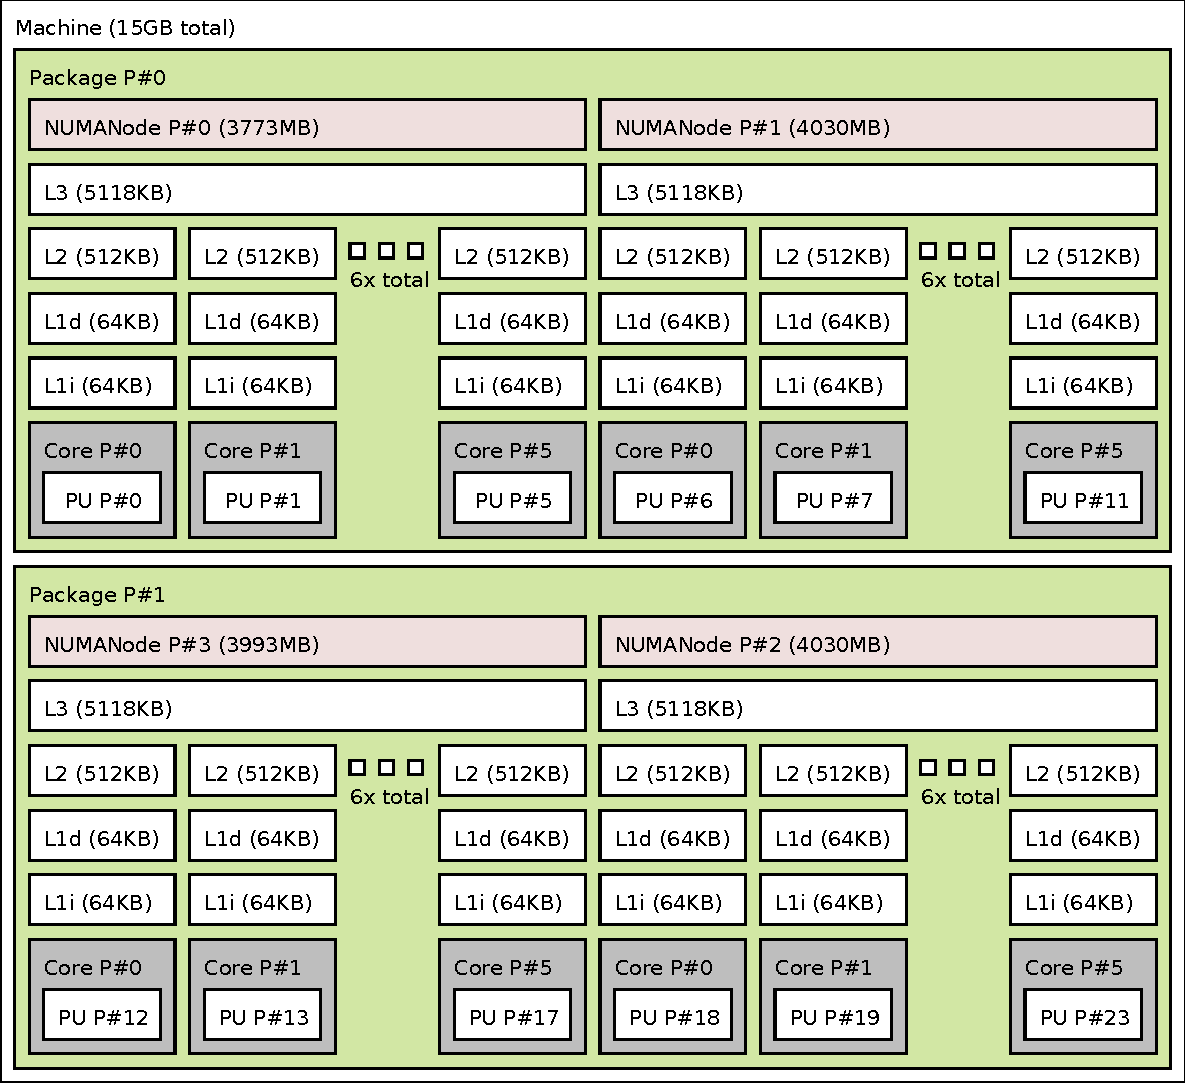
\includegraphics[width=0.8\textwidth]{Figures/paragon-topo.pdf}
	\linebreak
	\caption{Η τοπολογία του συστήματος Paragon.}
	\label{fig:paragon-topo}
\end{figure}


\section{Τοπολογία}
Η υλοποίηση των OpenMP places και OpenMP processor binding policies ελέγχθηκε για την ορθότητά της, δηλαδή  για το αν ικανοποιεί πλήρως τις προδιαγραφές του OpenMP, τόσο με ιδιόχειρα, όσο και με έτοιμα προγράμματα.   Τα έτοιμα προγράμματα ήταν μέρος ενός συνόλου προγραμμάτων ελέγχου ορθότητας τα οποία παρέχονται από τη βιβλιοθήκη \textit{GNU Offloading and Multi Processing Runtime Library} (libgomp) η οποία μεταξύ άλλων, υλοποιεί και τη διεπαφή προγραμματισμού εφαρμογών OpenMP που χρησιμοποιεί ο GCC.


\section{Barrier}
\label{sec:exp-barrier}
Η υλοποίηση του tree barrier ελέγχθηκε για την ορθότητά της με προγράμματα ελέγχου από τη βιβλιοθήκη libgomp και την \textit{OpenMP Validation Suite V 3.0} \cite{wang2012openmp, ompvalsuite3}. Ο λόγος όμως που αναπτύχθηκε ο tree barrier ήταν οι μειωμένες επιδόσεις του υπάρχοντα barrier του OMPi σε συστήματα NUMA, οπότε αφού εξασφαλίστηκε η ορθότητα της υλοποίησης, εστιάσαμε στο ζήτημα των επιδόσεων με τη χρήση μετροπρογραμμάτων.

Η \textit{EPCC OpenMP micro-benchmark suite} \cite{bull1999measuring} είναι ένα σύνολο μετροπρογραμμάτων (micro-benchmarks) τα οποία μετράνε το κόστος σε χρόνο (overhead) που απαιτείται για τη διεκπεραίωση λειτουργιών όπως ο συγχρονισμός (π.χ. barrier, κλειδαριές), η \textit{χρονοδρομολόγηση βρόχου} (loop scheduling) και οι πράξεις πινάκων. Η πιο πρόσφατη έκδοση (3.1) υποστηρίζει μέχρι και τις λειτουργίες που προδιαγράφει το OpenMP 3.0.

Τα πειράματα που πραγματοποιήθηκαν επικεντρώθηκαν στη μέτρηση του overhead του barrier, όσο το πλήθος των κόμβων NUMA που χρησιμοποιούνται αυξάνεται. Πιο συγκεκριμένα, ανατίθεται ένα δεδομένο πλήθος νημάτων ανά κόμβο, ενώ πραγματοποιούνται εκτελέσεις με 1 έως $N$ κόμβους, όπου $N$ το πλήθος των διαθέσιμων κόμβων του συστήματος. Με αυτό τον τρόπο ελέγχουμε κατά πόσο η εκάστοτε υλοποίηση barrier είναι κλιμακώσιμη. Οι υλοποιήσεις που συγκρίθηκαν είναι αυτές των μεταφραστών OMPi (κλασική και tree barrier), GCC, ICC και Clang.


\subsection{Parade}
Στα Σχήματα \ref{fig:bo-parade-sockets} α), γ) και ε) φαίνεται το overhead του κλασικού barrier του OMPi σε αντιπαραβολή με αυτό του νέου barrier όταν χρησιμοποιούνται 1 έως 4 κόμβοι, ενώ το πλήθος των νημάτων ανά κόμβο κυμαίνεται σε 8, 16 και 32. Επιπλέον, στα Σχήματα \ref{fig:bo-parade-sockets} β), δ) και στ) έχουν προστεθεί οι γραφικές παραστάσεις του overhead των μεταφραστών GCC, ICC και Clang.

Επειδή στις συγκεκριμένες εκδόσεις των μεταφραστών μόνο οι OMPi και ICC υποστηρίζουν το αφηρημένο όνομα \texttt{numa\_domains}, για την ανάθεση των νημάτων σε επεξεργαστές και συνεπώς σε κόμβους χρησιμοποιήθηκε το αφηρημένο όνομα \texttt{sockets} το οποίο στην περίπτωση του Parade είναι ταυτόσημο με το όνομα \texttt{numa\_domains}. Πιο συγκεκριμένα, στις μεταβλητές περιβάλλοντος του OpenMP ανατέθηκαν οι εξής τιμές: \texttt{OMP\_PLACES="sockets($N$)"}, \texttt{OMP\_NUM\_THREADS="$T$"} και \texttt{OMP\_PROC\_BIND="close"}, όπου $N$ το πλήθος των sockets/κόμβων που χρησιμοποιούνται κάθε φορά (1, 2, 3 και 4) και $T$ το συνολικό πλήθος των νημάτων που προκύπτει ως $N \times T_n$, με το $T_n$ να αναπαριστά το πλήθος των νημάτων που θέλουμε να χρησιμοποιηθούν σε κάθε κόμβο (8, 16 και 32). Η πολιτική \texttt{close} χρησιμοποιήθηκε για την ισοκατανομή των $T$ νημάτων στους $N$ κόμβους, δηλαδή για την ανάθεση $T_n = T/N$ νημάτων ανά κόμβο. Με αυτό τον τρόπο, ανατίθενται $T_n$ νήματα σε κάθε κόμβο, χωρίς όμως να γνωρίζουμε ακριβώς σε ποιούς επεξεργαστές του κόμβου θα ανατεθούν τα $T_n$ νήματα, καθώς η ακριβής τοποθέτηση των νημάτων εξαρτάται από τη βιβλιοθήκη νημάτων που χρησιμοποιεί η κάθε υλοποίηση και πιθανώςc και από το λειτουργικό σύστημα.

Αυτό που παρατηρούμε βάσει του Σχήματος \ref{fig:bo-parade-sockets}, είναι ο μεγάλος ρυθμός αύξησης του overhead στην περίπτωση του παλιού barrier του OMPi. Σε αντίθεση, ο νέος barrier, στην περίπτωση του ενός κόμβου επιδεικνύει ελαφρώς μεγαλύτερο overhead σε σχέση με τον παλιό, ενώ για δύο ή περισσότερους κόμβους ο ρυθμός αύξησης είναι ιδιαίτερα μικρός. Το overhead του tree barrier όταν χρησιμοποιούνται δύο κόμβοι είναι σαφώς πιο αυξημένο σε σχέση με όταν χρησιμοποιείται ένας κόμβος, φαινόμενο πλήρως δικαιολογημένο καθώς στην πρώτη περίπτωση πραγματοποιούνται απομακρυσμένες προσβάσεις μνήμης και ο αλγόριθμος barrier είναι πιο πολύπλοκος. Όταν χρησιμοποιούνται 8 νήματα ανά κόμβο (Σχήματα \ref{fig:bo-parade-sockets} α) και β)) παρατηρούμε ότι ο παλιός barrier πλησιάζει το overhead του νέου, κάτι που πιθανώς συμβαίνει λόγω του μικρού πλήθους νημάτων (Η αξιοποίηση των H/W threads του κόμβου ανέρχεται το πολύ στο $25\%$).

\begin{figure}[htbp]
    \centering
    \begin{minipage}{0.5\textwidth}
        \centering
        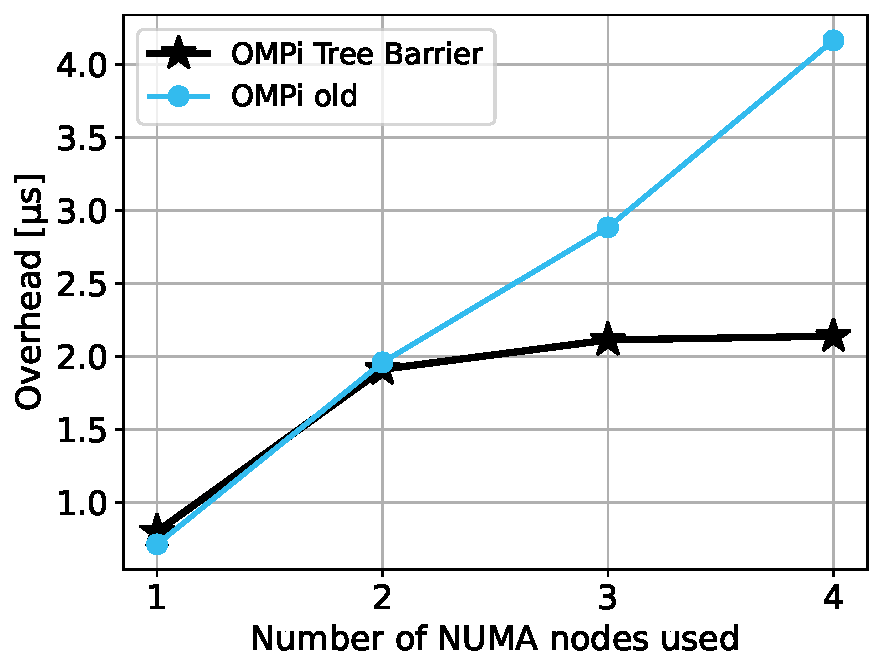
\includegraphics[width=1\textwidth]{Figures/parade-epcc/ompionly_sockets_tpn-8_close.pdf}
		α)
    \end{minipage}\hfill
     \begin{minipage}{0.5\textwidth}
        \centering
        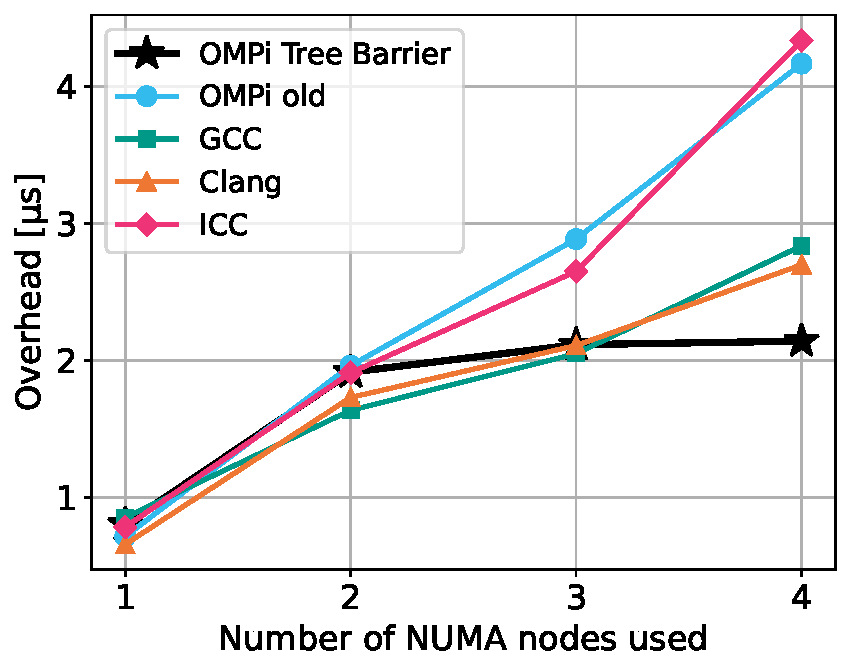
\includegraphics[width=1\textwidth]{Figures/parade-epcc/sockets_tpn-8_close.pdf}
		β)
    \end{minipage}
    \newline
    \begin{minipage}{0.5\textwidth}
        \centering
        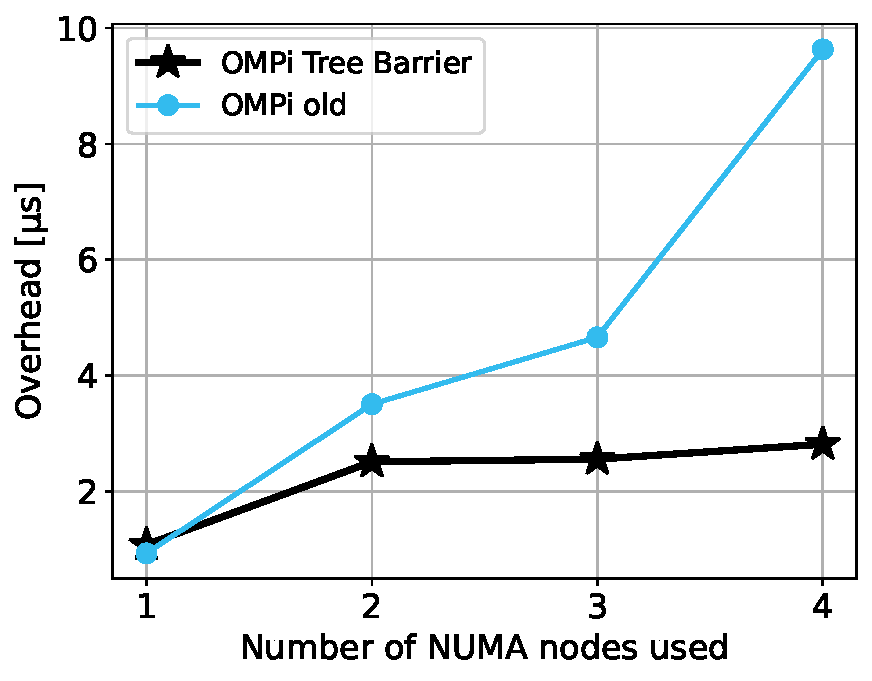
\includegraphics[width=1\textwidth]{Figures/parade-epcc/ompionly_sockets_tpn-16_close.pdf}
        γ)
    \end{minipage}\hfill
    \begin{minipage}{0.5\textwidth}
        \centering
        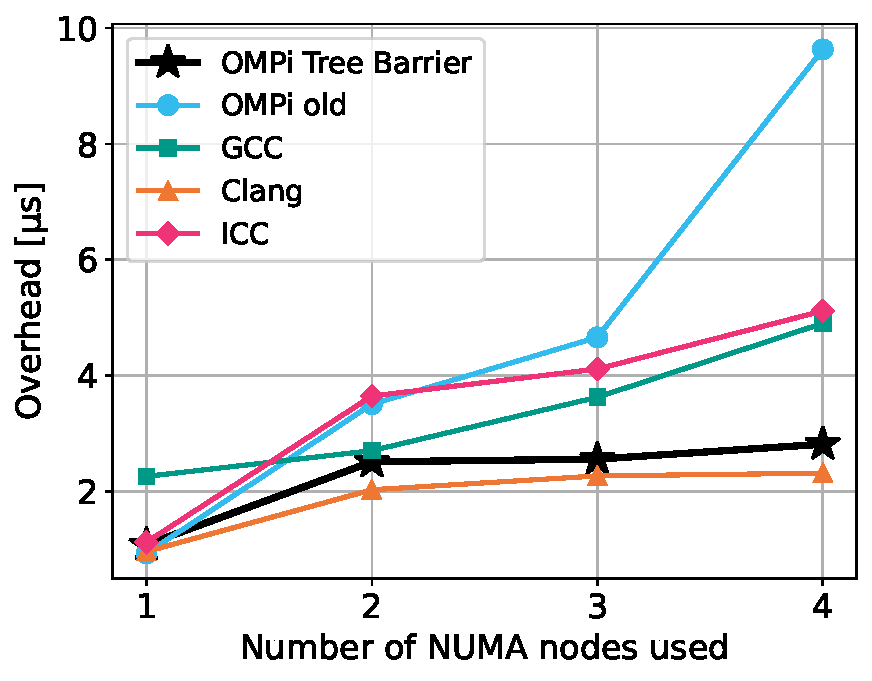
\includegraphics[width=1\textwidth]{Figures/parade-epcc/sockets_tpn-16_close.pdf}
        δ)
    \end{minipage}
    \newline
    \begin{minipage}{0.5\textwidth}
        \centering
        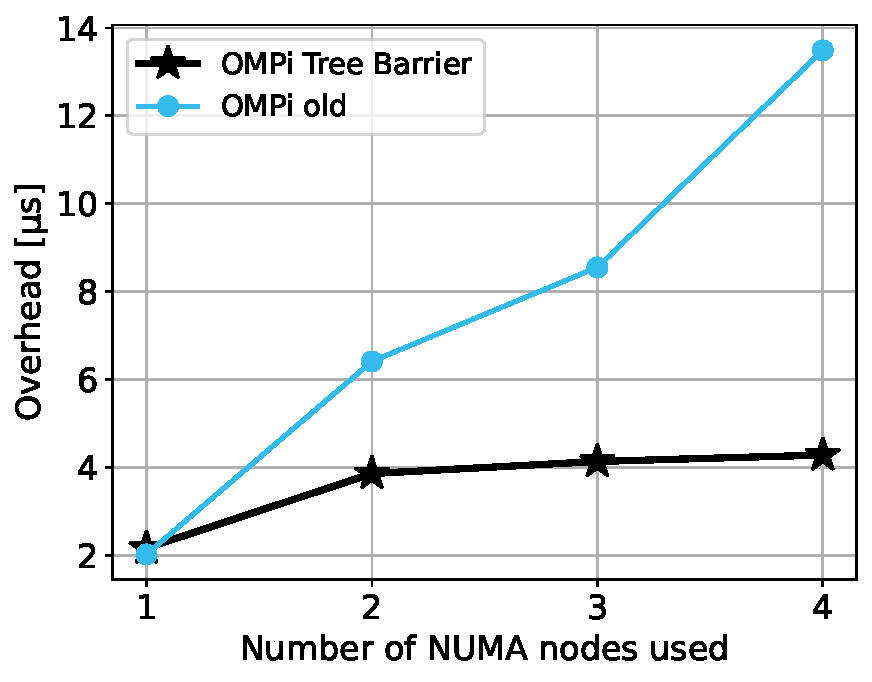
\includegraphics[width=1\textwidth]{Figures/parade-epcc/ompionly_sockets_tpn-32_close.pdf}
        ε)
    \end{minipage}\hfill
    \begin{minipage}{0.5\textwidth}
        \centering
        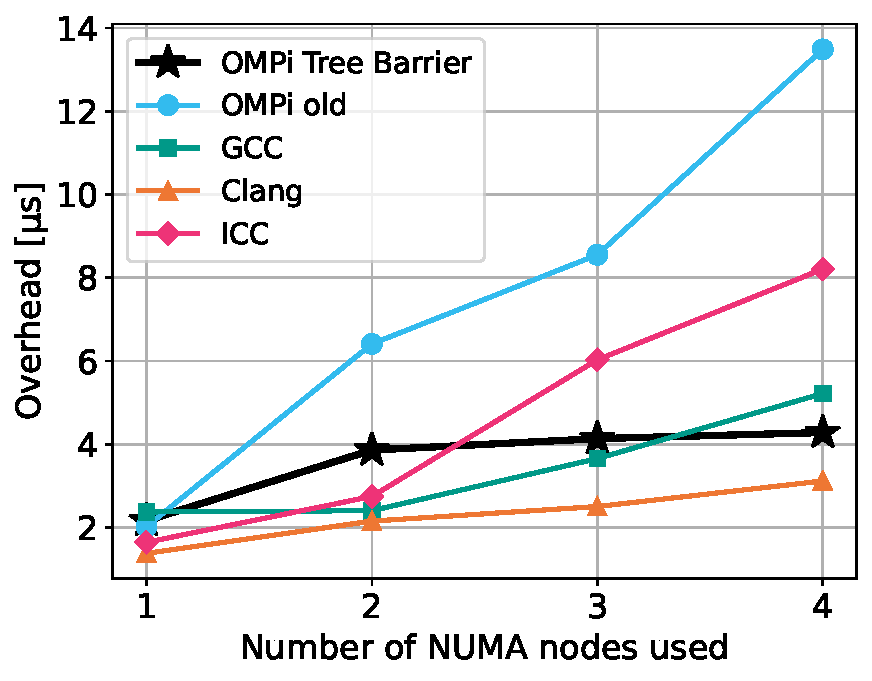
\includegraphics[width=1\textwidth]{Figures/parade-epcc/sockets_tpn-32_close.pdf}
        στ)
    \end{minipage}
    \newline \newline
    {\small α), β) 8 νήματα ανά κόμβο, γ), δ) 16 νήματα ανά κόμβο, ε), στ) 32 νήματα ανά κόμβο}
    \caption{Barrier overhead στον Parade (ανάθεση νημάτων ανά socket).}
    \label{fig:bo-parade-sockets}
\end{figure}

Κατά τη διάρκεια διεξαγωγής των παραπάνω πειραμάτων, παρατηρήθηκαν μεγάλες και μη αναμενόμενες διακυμάνσεις στο overhead, ειδικά στην περίπτωση του ICC και του Clang. Για παράδειγμα, το overhead για δύο κόμβους ήταν πολύ μεγαλύτερο σε σχέση με αυτό για τρεις ή τέσσερις κόμβους. Ο λόγος που συμβαίνει αυτό κατά πάσα πιθανότητα έγγειται στο γεγονός ότι υπάρχει έλλειψη ελέγχου στο πώς ανατίθενται τα νήματα στα H/W threads του socket, καθώς παρατηρήθηκε ότι ακόμα και 3 νήματα εκτελούνταν στο ίδιο H/W thread ενώ θα μπορούσαν να ανατεθούν σε διαφορετικά. Παρόλα αυτά, η χρήση πιο περιοριστικών τρόπων ανάθεσης νημάτων (π.χ. ανά core ή H/W thread) οδηγεί σε χειρότερες ή καλύτερες επιδόσεις ανάλογα με τον κάθε μεταφραστή, καθιστώντας με αυτό τον τρόπο δυσχερή τη δίκαιη σύγκριση μεταξύ τους.

Ενδεικτικά, στο Σχήμα \ref{fig:bo-parade-topothreads} φαίνονται οι μετρήσεις οι οποίες έγιναν χρησιμοποιώντας πιο περιοριστικούς τρόπους ανάθεσης νημάτων σε επεξεργαστές. Πιο συγκεκριμένα, αντί να ανατεθούν $T_n$ (8, 16 και 32) νήματα στο σύνολο των H/W threads του κάθε κόμβου, ανατέθηκε ένα νήμα σε ένα μόνο H/W thread με τέτοιο τρόπο ώστε η κατανομή εντός του κόμβου να είναι αραιή και να μη χρησιμοποιούνται H/W threads που ανήκουν σε γειτονικά places. Η ανάθεση αυτή επιτεύχθηκε με τον ακόλουθο τρόπο. Αρχικά ορίστηκαν τα OpenMP places με τη χρήση ρητής λίστας η οποία περιγράφει κάθε φορά τα αναγνωριστικά των επεξεργαστών που περιέχονται σε 1, 2, 3 και 4 κόμβους και άρα το μέγεθος του place partition ισούται με $P = N \times 32$, όπου $N$ το πλήθος των κόμβων που χρησιμοποιούνται κάθε φορά. Η ρητή λίστα βασίστηκε στην τοπολογία όπως αυτή παρέχεται από τη βιβλιοθήκη hwloc που είδαμε νωρίτερα στην Υποενότητα \ref{ssec:hwloc}.

\begin{figure}[htbp]
    \centering
    \begin{minipage}{0.5\textwidth}
        \centering
        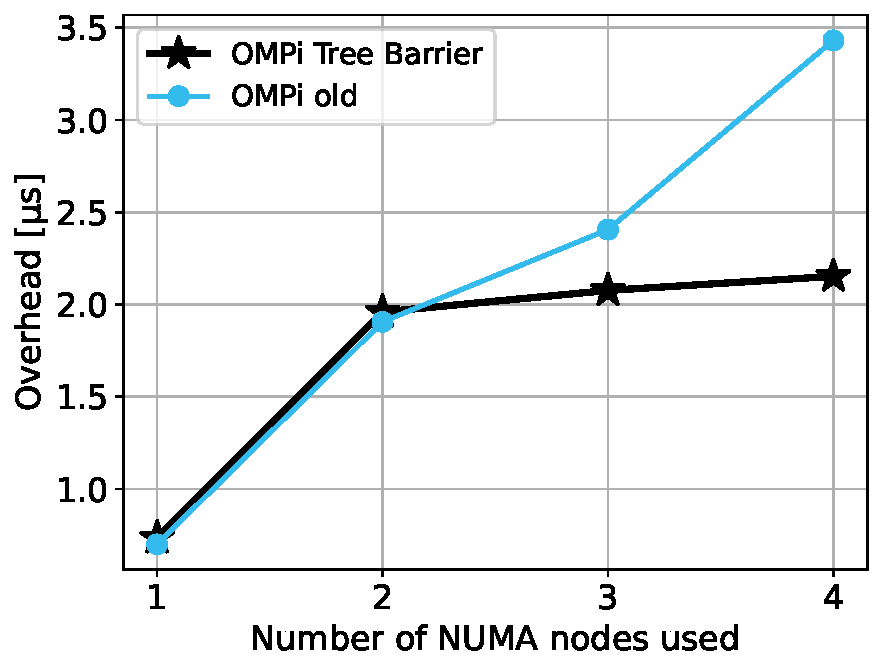
\includegraphics[width=1\textwidth]{Figures/parade-epcc/ompionly_topothreads_tpn-8_spread.pdf}
		α)
    \end{minipage}\hfill
     \begin{minipage}{0.5\textwidth}
        \centering
        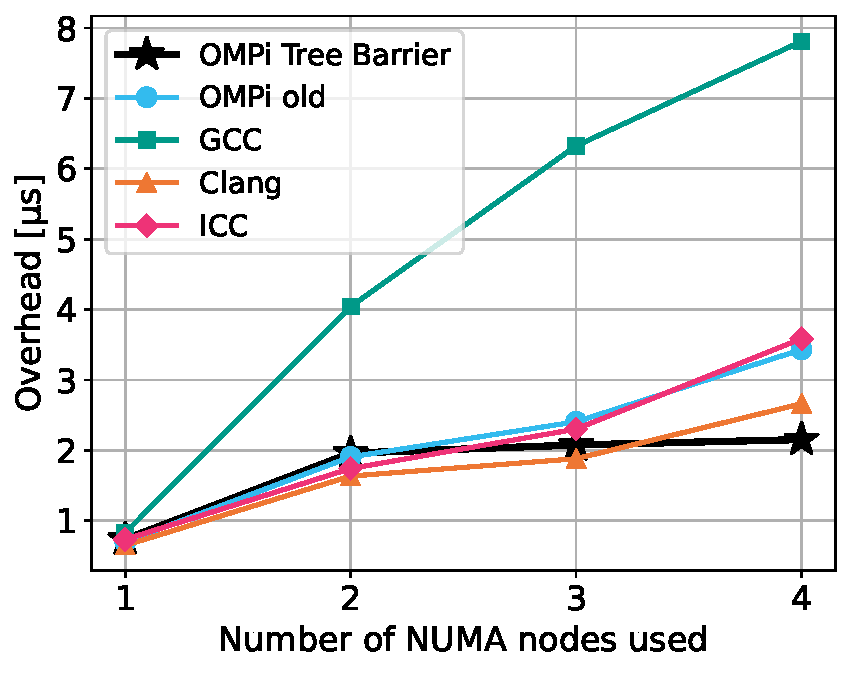
\includegraphics[width=1\textwidth]{Figures/parade-epcc/topothreads_tpn-8_spread.pdf}
		β)
    \end{minipage}
    \newline
    \begin{minipage}{0.5\textwidth}
        \centering
        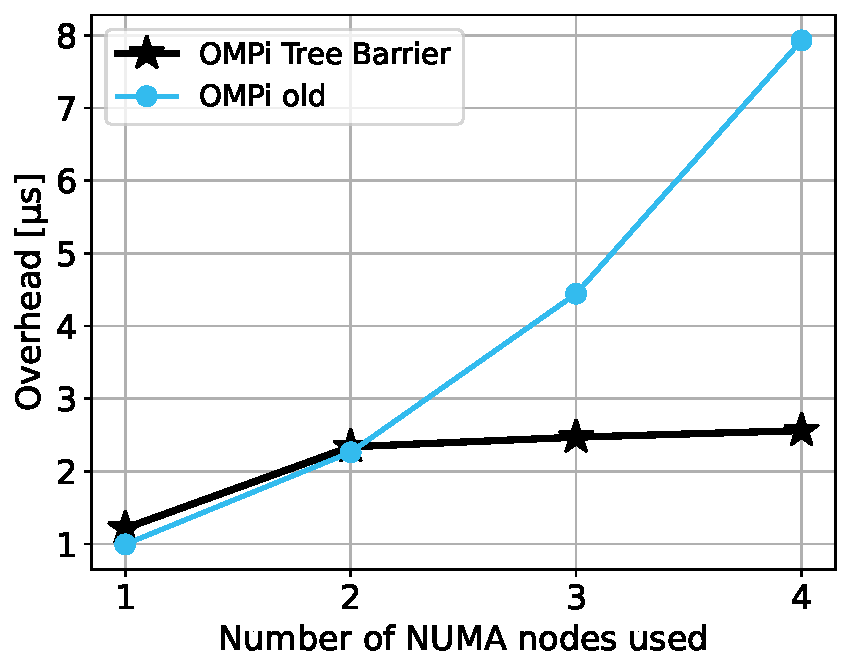
\includegraphics[width=1\textwidth]{Figures/parade-epcc/ompionly_topothreads_tpn-16_spread.pdf}
        γ)
    \end{minipage}\hfill
    \begin{minipage}{0.5\textwidth}
        \centering
        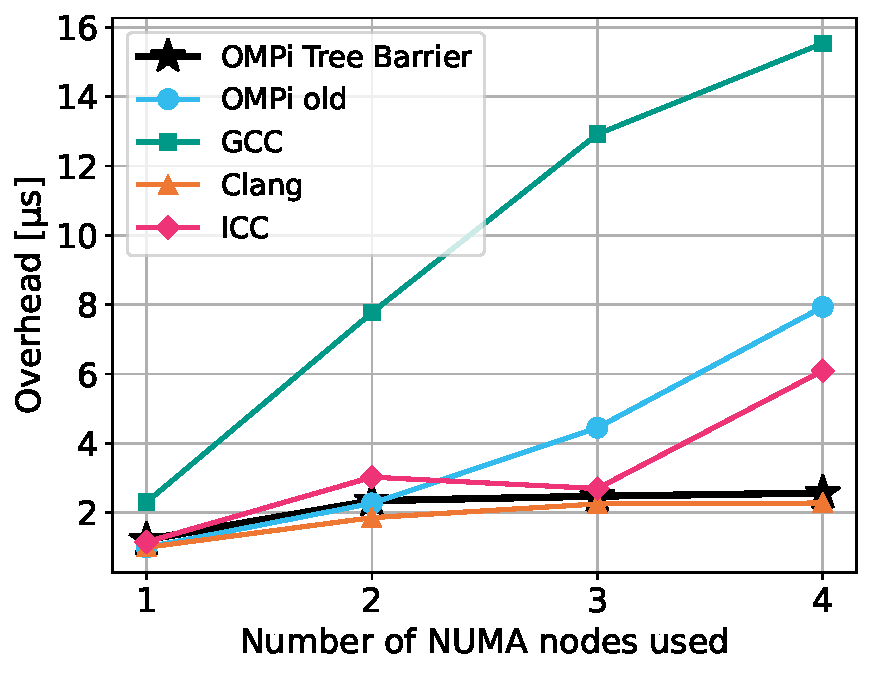
\includegraphics[width=1\textwidth]{Figures/parade-epcc/topothreads_tpn-16_spread.pdf}
        δ)
    \end{minipage}
    \newline
    \begin{minipage}{0.5\textwidth}
        \centering
        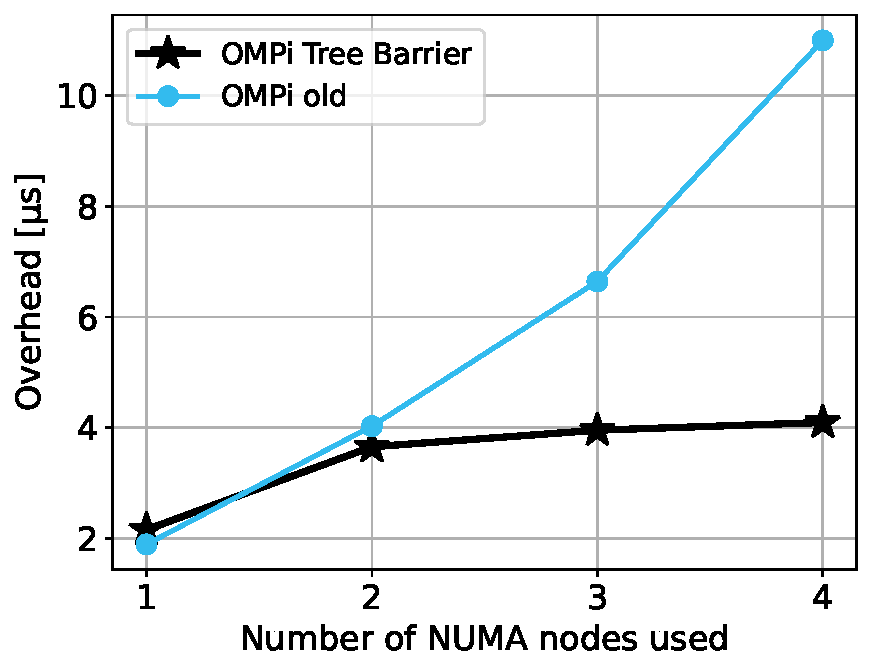
\includegraphics[width=1\textwidth]{Figures/parade-epcc/ompionly_topothreads_tpn-32_close.pdf}
        ε)
    \end{minipage}\hfill
    \begin{minipage}{0.5\textwidth}
        \centering
        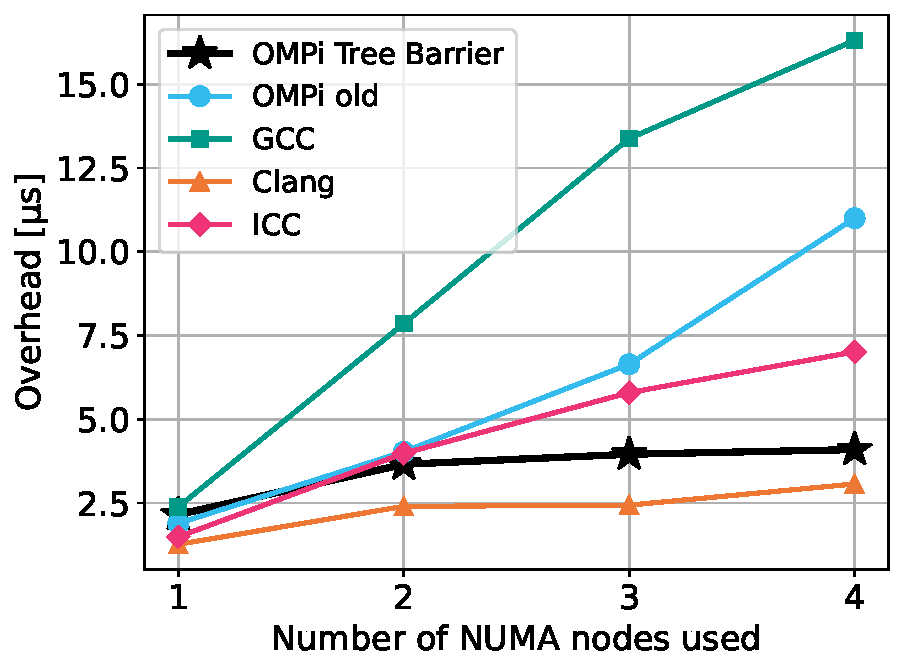
\includegraphics[width=1\textwidth]{Figures/parade-epcc/topothreads_tpn-32_close.pdf}
        στ)
    \end{minipage}
    \newline \newline
    {\small α), β) 8 νήματα ανά κόμβο, γ), δ) 16 νήματα ανά κόμβο, ε), στ) 32 νήματα ανά κόμβο}
    \caption{Barrier overhead στον Parade (ανάθεση νημάτων σε H/W threads).}
    \label{fig:bo-parade-topothreads}
\end{figure}

Η χρήση αφηρημένου ονόματος αποφεύχθηκε καθώς ο κάθε μεταφραστής μετασχηματίζει με διαφορετικό τρόπο το αφηρημένο όνομα σε αναγνωριστικά επεξεργαστών. Για παράδειγμα, στην περίπτωση του αφηρημένου ονόματος \texttt{threads}, ο GCC τοποθετεί στο place partition με κυκλικό τρόπο (round-robin) ένα H/W thread ανά κόμβο. Συνεπώς, αν ο χρήστης επιλέξει ως processor binding policy την \texttt{close}, νήματα που θα τοποθετηθούν σε γειτονικά places, θα καταλήξουν σε διαφορετικούς κόμβους NUMA.

Στη συνέχεια, ως πολιτική επιλέχθηκε η \texttt{spread} καθώς μπορεί να ισοκατανήμει με αραιό τρόπο τα $T$ νήματα στα $P \geq T$ places, τοποθετώντας ένα νήμα ανά $32 / T_n$ (4, 2 και 1) H/W threads και συνεπώς τοποθετώντας συνολικά 8, 16 και 32 νήματα ανά κόμβο. Στη μεταβλητή \texttt{OMP\_NUM\_THREADS}, όπως και προηγουμένως, ανατέθηκε η τιμή $T$ η οποία αντιστοιχεί στο συνολικό πλήθος των νημάτων και προκύπτει ως $N \times T_n$, με το $T_n$ να αναπαριστά το πλήθος των νημάτων που θέλουμε να χρησιμοποιηθούν σε κάθε κόμβο (8, 16 και 32).

Βάσει του Σχήματος \ref{fig:bo-parade-topothreads} και συγκριτικά με τον προηγούμενο τρόπο ανάθεσης\footnote{Αφηρημένο όνομα \texttt{sockets}.} παρατηρούμε τα ακόλουθα. Ο tree barrier έχει σχεδόν τις ίδιες επιδόσεις, ενώ ο παλιός barrier έχει καλύτερες επιδόσεις για δύο κόμβους και πλησιάζουν εκείνες του tree barrier, όμως για τρεις και τέσσερις κόμβους το overhead αυξάνεται με μεγάλο ρυθμό. Ο GCC επιδεικνύει πολύ μεγαλύτερο overhead για δύο ή περισσότερους κόμβους, γεγονός που τον οδηγεί εκτός συναγωνισμού. Οι ICC και Clang παρουσιάζουν άλλες φορές καλύτερες και άλλες φορές χειρότερες επιδόσεις. Από τα παραπάνω, γίνεται αντιληπτή η επίδραση στο χρόνο εκτέλεσης που μπορεί να έχει ο έλεγχος του τρόπου ανάθεσης των νημάτων σε επεξεργαστές. Τέλος, παρόλο που το φαινόμενο των μεγάλων και απρόσμενων διακυμάνσεων του overhead αμβλύνθηκε σημαντικά, η επιρροή κάποιων μεταφραστών προς το χειρότερο αποτρέπει την περαιτέρω χρήση τόσο περιοριστικών τρόπων ανάθεσης.

Από το σύνολο των παραπάνω παρατηρήσεων συμπεραίνουμε ότι ο tree barrier διατηρεί τον μικρό ρυθμό αύξησης του overhead για δύο ή περισσότερους κόμβους, ανεξάρτητα από τον τρόπο ανάθεσης των νημάτων σε επεξεργαστές. Αυτή η συμπεριφορά μπορεί να παρατηρηθεί μόνο στον Clang, με εξαίρεση την περίπτωση που χρησιμοποιούνται 8 νήματα ανά κόμβο, κατά την οποία ο Clang εμφανίζει μεγαλύτερο ρυθμό αύξησης κατά τη μετάβαση από τους τρεις στους τέσσερις κόμβους.

\subsection{Paragon}
Στον Paragon, μετρήθηκε το overhead του barrier κάθε μεταφραστή όταν χρησιμοποιούνται 1 έως 4 κόμβοι και 6 νήματα ανά κόμβο, με ανάλογο τρόπο με αυτόν που χρησιμοποιήθηκε στον Parade. Η μόνη διαφοροποίηση αφορούσε τον ορισμό του place partition μέσω της μεταβλητής περιβάλλοντος \texttt{OMP\_PLACES}. Πιο συγκεκριμένα, εκτός από το αφηρημένο όνομα \texttt{numa\_domains} ήταν αδύνατο να χρησιμοποιηθεί και το αφηρημένο όνομα \texttt{sockets} για την τοποθέτηση νημάτων σε κόμβους, καθώς κάθε ολοκληρωμένο κύκλωμα επεξεργαστή περιέχει δύο κόμβους και συνεπώς τα δύο αφηρημένα ονόματα δεν είναι ταυτόσημα. Επειδή όμως στο συγκεκριμένο σύστημα όλοι οι μεταφραστές μετασχηματίζουν με τον ίδιο τρόπο τα αφηρημένα ονόματα σε αναγνωριστικά επεξεργαστών\footnote{Οι ICC και Clang εσφαλμένα θεωρούν ότι κάθε επεξεργαστής διαθέτει ένα μόνο core αντί για δώδεκα, γεγονός που θεωρήθηκε ως σφάλμα (bug) και αγνοήθηκε.}, είναι εφικτός ο μονοσήμαντος ορισμός του αρχικού place partition με τη χρήση ρητής λίστας. Συνεπώς, σε αντίθεση με τον Parade, αντί για τoν ορισμό του place partition ως \texttt{sockets($N$)}, όπου $N$ το πλήθος τον κόμβων που χρησιμοποιούνται κάθε φορά (1,2,3 και 4), χρησιμοποιήθηκε ρητή λίστα που περιγράφει $N$ places, με κάθε place να περιέχει τα αναγνωριστικά των επεξεργαστών που ανήκουν στον $N$-οστό κόμβο.

Στο Σχήμα \ref{fig:bo-paragon-toponodes} φαίνονται τα αποτελέσματα των παραπάνω μετρήσεων. Βάσει των μετρήσεων αυτών παρατηρούμε ότι τα overheads των OMPi, GCC και ICC αυξάνουν περίπου γραμμικά και σχεδόν συγκλίνουν για πλήθος τεσσάρων κόμβων. Ο Clang φαίνεται να κλιμακώνει καλύτερα για τρεις και τέσσερις κόμβους από τους OMPi, GCC και ICC, αλλά όχι το ίδιο αποδοτικά όπως συνέβαινε στον Parade. Ο OMPi tree barrier επιδεικνύει την καλύτερη επίδοση για τρεις και τέσσερις κόμβους, με το overhead να αυξάνει με πολύ μικρό ρυθμό όσο αυξάνεται το πλήθος των κόμβων, φαινόμενο που παρατηρήθηκε και στον Parade. Επιπλέον, παρατηρούμε ο tree barrier έχει οριακά μεγαλύτερο overhead σε σχέση με τον κλασικό barrier του OMPi, όχι μόνο για ένα κόμβο αλλά και για δύο, κάτι που πιθανώς συμβαίνει λόγω του μικρού πλήθους νημάτων. Τέλος, όπως και στον Parade, βλέπουμε ότι η συνολική επίδοση του tree barrier καθορίζεται από το overhead που εισάγεται κατά τη μετάβαση από έναν κόμβο σε δύο.

Επιπλέον των παραπάνω μετρήσεων στις οποίες τα νήματα που τοποθετούνται σε κάθε κόμβο ανατίθενται στο σύνολο των επεξεργαστών που τον αποτελούν, πραγματοποιήθηκε ανάθεση κάθε νήματος σε συγκεκριμένο H/W thread του κόμβου, παρόλο που δεν παρατηρήθηκαν διακυμάνσεις όπως συνέβη στον Parade. Στο Σχήμα \ref{fig:bo-paragon-topothreads} φαίνονται οι μετρήσεις που έγιναν χρησιμοποιώντας πιο περιοριστικούς τρόπους ανάθεσης και στις οποίες παρατηρούμε ότι η επίδοση των μεταφραστών είναι σε μεγάλο βαθμό ίδια, πλην ελάχιστων μικροδιαφορών, όπως για παράδειγμα το μικρότερο overhead των ICC και Clang για τέσσερις κόμβους.

%Στον Paragon, εκτός από το αφηρημένο όνομα \texttt{numa\_domains} ήταν αδύνατο να χρησιμοποιηθεί και το αφηρημένο όνομα \texttt{sockets} για την τοποθέτηση νημάτων σε κόμβους NUMA, καθώς κάθε ολοκληρωμένο κύκλωμα επεξεργαστή περιέχει δύο κόμβους και συνεπώς τα δύο αφηρημένα ονόματα δεν είναι ταυτόσημα. Επιπλέον, όλοι οι μεταφραστές μετασχηματίζουν με τον ίδιο τρόπο τα αφηρημένα ονόματα σε αναγνωριστικά επεξεργαστών\footnote{Οι ICC και Clang εσφαλμένα θεωρούν ότι κάθε επεξεργαστής διαθέτει ένα μόνο core αντί για δώδεκα, γεγονός που θεωρήθηκε ως σφάλμα (bug) και αγνοήθηκε.}, κάτι που επιτρέπει τον μονοσήμαντο ορισμό του place partition ως ρητή λίστα.

\begin{figure}[htbp]
    \centering
    \begin{minipage}{0.48\textwidth}
        \centering
        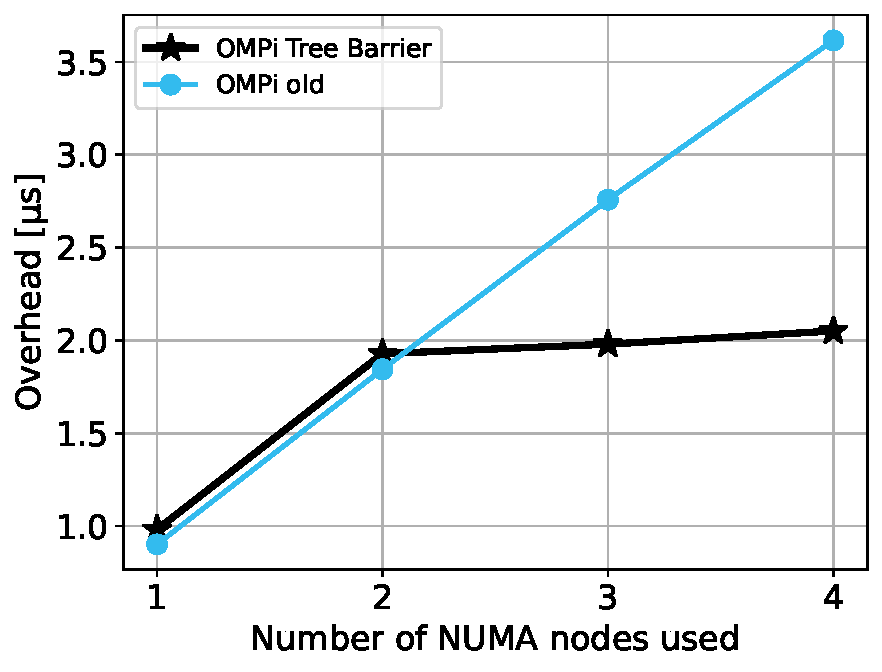
\includegraphics[width=1\textwidth]{Figures/paragon-epcc/ompionly_toponodes_tpn-6_close.pdf}
    \end{minipage}\hfill
    \begin{minipage}{0.48\textwidth}
        \centering
        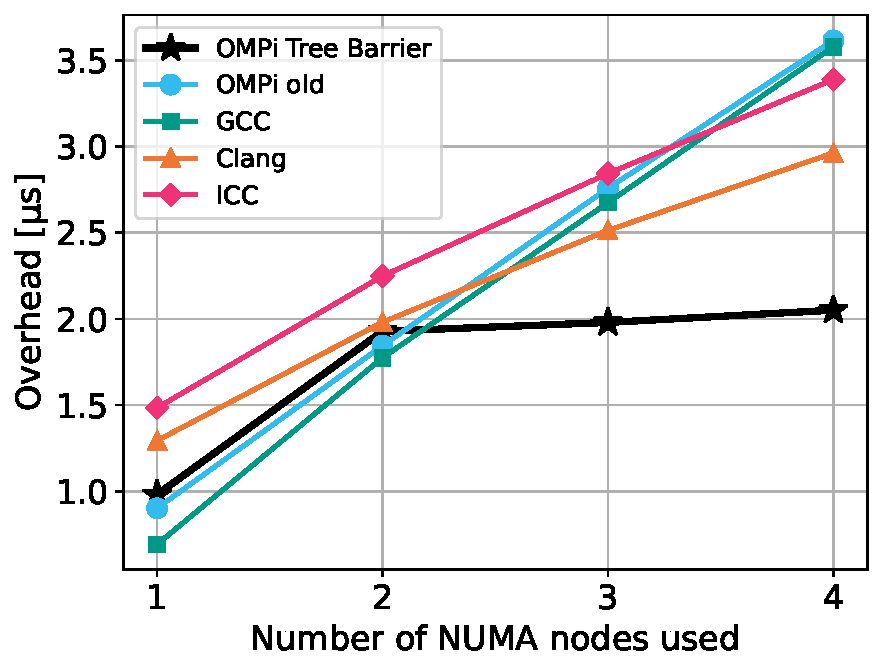
\includegraphics[width=1\textwidth]{Figures/paragon-epcc/toponodes_tpn-6_close.pdf}
    \end{minipage}
    \newline \newline
    {\small Χρησιμοποιήθηκαν 6 νήματα ανά κόμβο.}
    \caption{Barrier overhead στον Paragon (ανάθεση νημάτων σε κόμβους).}
    \label{fig:bo-paragon-toponodes}
\end{figure}

\begin{figure}[htbp]
    \centering
    \begin{minipage}{0.48\textwidth}
        \centering
        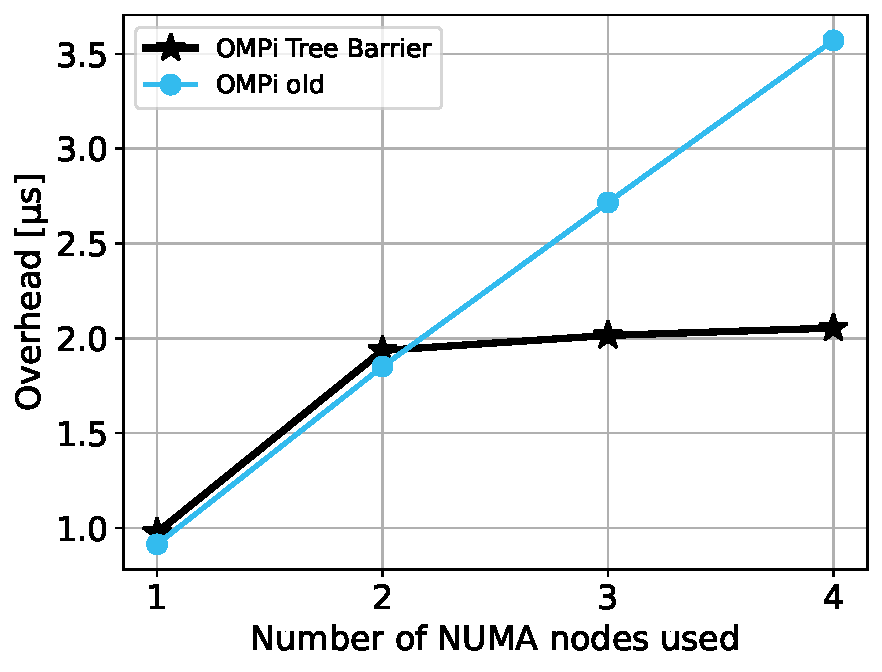
\includegraphics[width=1\textwidth]{Figures/paragon-epcc/ompionly_topothreads_tpn-6_close.pdf}
    \end{minipage}\hfill
    \begin{minipage}{0.48\textwidth}
        \centering
        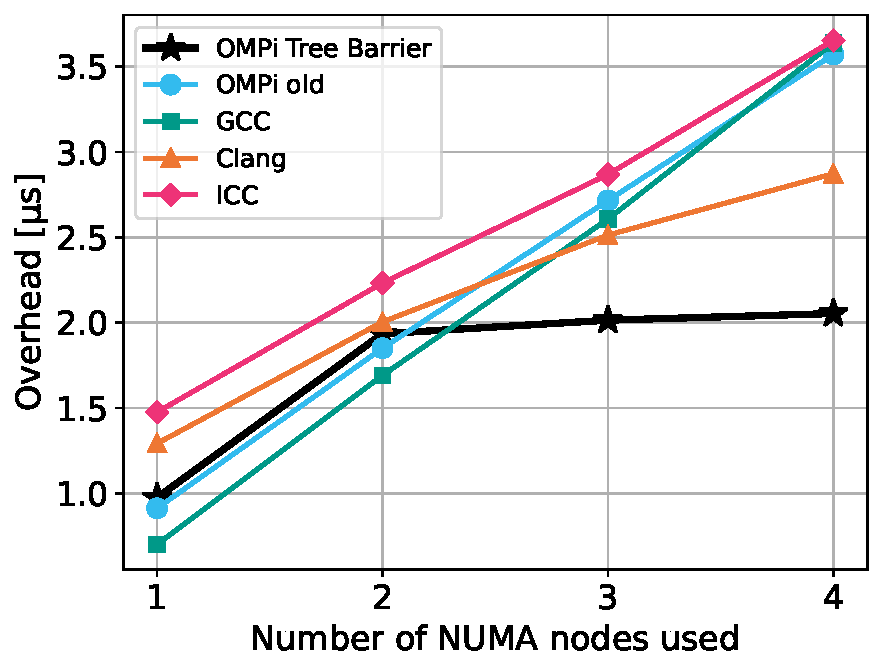
\includegraphics[width=1\textwidth]{Figures/paragon-epcc/topothreads_tpn-6_close.pdf}
    \end{minipage}
    \newline \newline
    {\small Χρησιμοποιήθηκαν 6 νήματα ανά κόμβο.}
    \caption{Barrier overhead στον Paragon (ανάθεση νημάτων σε H/W threads).}
    \label{fig:bo-paragon-topothreads}
\end{figure}

%Βάσει των μετρήσεων αυτών παρατηρούμε ότι τα overheads των OMPi, GCC και ICC αυξάνουν περίπου γραμμικά και σχεδόν συγκλίνουν για πλήθος τεσσάρων κόμβων. Ο Clang φαίνεται ότι κλιμακώνει καλύτερα για τρεις και τέσσερις κόμβους από τους OMPi, GCC και ICC, αλλά όχι το ίδιο αποδοτικά όπως συνέβαινε στον Parade. Ο OMPi tree barrier επιδεικνύει την καλύτερη επίδοση για τρεις και τέσσερις κόμβους, με το overhead να αυξάνει με πολύ μικρό ρυθμό όσο αυξάνεται το πλήθος των κόμβων, φαινόμενο που παρατηρήθηκε και στον Parade. Επιπλέον, παρατηρούμε ο tree barrier έχει οριακά μεγαλύτερο overhead σε σχέση με τον κλασικό barrier του OMPi, όχι μόνο για ένα κόμβο αλλά και για δύο, κάτι που πιθανώς συμβαίνει λόγω του μικρού πλήθους νημάτων.
